\section{Approaches}

To achieve broader usage it is important to require few if any changes to either the VR toolkit or the third party scientific visualization software, and to work as close as possible to the standard application development workflow.
For VTK, this was accomplished by adding new features that fit within the existing architecture. 
VTK provides a well-defined rendering pipeline through the \texttt{RenderWindow}, \texttt{Renderer}, \texttt{Camera}, \texttt{Actor}, and \texttt{Mapper} classes.
This precise pipeline definition and clear-cut API of VTK enabled us to primarily build upon
existing code.
In the next section we cover details on these components from the architecture point of view.
In the implementation sub-section, we provide in-depth details of features we implemented to support configurable immersive scientific visualization applications. 

\subsection{OpenGL context sharing}

Traditionally, VTK creates and manages its own OpenGL context and the data objects within the scene.
The objective of this work is to bring the high-quality scientific visualization computing and rendering capabilities of VTK to virtual reality environments in a way that is easier to develop and maintain.
By bringing VTK into virtual environments created by interface-specific tools such as GLUT, VRUI, and FreeVR, we are providing the tools necessary to build interactive, 3D scientific visualizations to the developers of the virtual reality community.

\subsubsection{Architecture}

Integrating VTK into external rendering systems required overriding some of the behavior of the \texttt{vtkRenderWindow}, \texttt{vtkRenderer}, and \texttt{vtkCamera} classes.
A \texttt{Renderer} is attached to a \texttt{RenderWindow}, a \texttt{Mapper} to an \texttt{Actor}, and a \texttt{Camera} to a \texttt{Renderer}.
In a typical VTK application the \texttt{RenderWindow} class is responsible for creating a rendering context, and defining width and height of the visualization viewport.
The \texttt{Renderer} class is responsible for rendering one-or-more
\texttt{Actor}s and managing the viewport within the \texttt{RenderWindow}.
The \texttt{Actor} class is a drawable entity, which uses a \texttt{Mapper} to render specific data within a \texttt{Renderer}.
Figure \ref{fig:vtkRenderPipeline} shows the classes and interactions between them.

Each of these components has its corresponding derived classes that implement the API using OpenGL, VTK's underlying graphics API.
Using OpenGL provides VTK with the ability to use hardware acceleration that ultimately leads to better visualizations and near real-time performance as required by many interactive applications especially ones that are designed for immersive environments.
Each component of VTK participates in a specific way and communicates with other components via the public API.
For instance, the \texttt{RenderWindow} typically creates the context in which
\texttt{Renderer} draws drawable entities, i.e. \texttt{Actor}s.
%A \texttt{RenderWindow} can have one or more \texttt{Renderer}s.
%Each \texttt{Renderer} can make a decision on whether or not it should reset the buffers such as color or depth to its initial state while rendering one-or-more actors. 

% WRS: the figure could benefit by having what type of data flows between
%   the modules (like the colors of AVS).
%  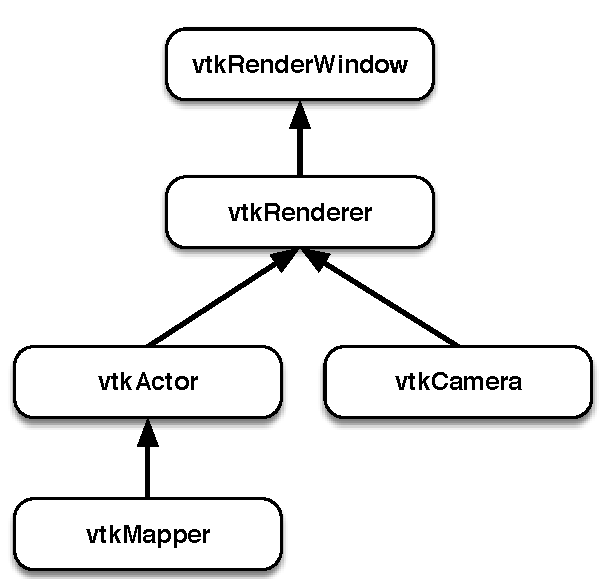
\includegraphics[width=\linewidth, scale=0.5]{images/vtkRenderPipeline.pdf}
\begin{figure}[h!]
  \centering
  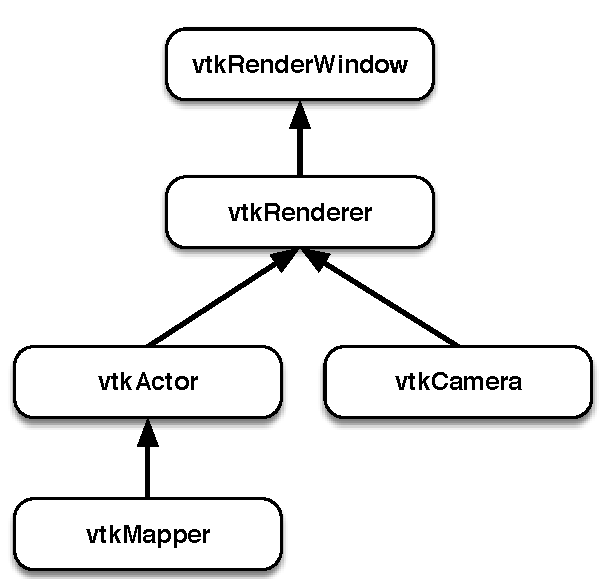
\includegraphics[scale=0.5]{images/vtkRenderPipeline.pdf}
  \caption{vtkRenderWindow, vtkRenderer, vtkCamera, vtkActor, and vtkMapper interaction diagram.}
  \label{fig:vtkRenderPipeline}
\end{figure}

Since \texttt{vtkRenderWindow} typically creates the context, and \texttt{vtkRenderer} controls objects of a scene in a given viewport, the rendering pipeline is constructed with properties and other attributes set specifically to support this most general use case.
% WRS: (above sentence) controls how?
However, in the case of external environments, the context is created outside of VTK, and non-VTK graphical elements (such as the GUI) may be rendered before or after the VTK rendering.
In addition, the environment may render its own visualization objects in the same context.
To handle this situation, we have introduced a new module in VTK called \texttt{vtkRenderingExternal} that comprises four new classes: \texttt{vtkExternalOpenGLRenderWindow}, \texttt{vtkExternalOpenGLRenderer}, \texttt{vtkExternalOpenGLCamera} and \texttt{ExternalVTKWidget}. 

\textbf{\texttt{vtkExternalOpenGLRenderWindow}} - This class is an extension to
the \texttt{vtkGenericOpenGLRenderWindow} class, which provides a
platform-agnostic VTK OpenGL window.
The external render window class prevents a new VTK render window from being
created and, instead, uses an existing OpenGL context.
It is also responsible for fetching stereo parameters from the parent OpenGL
application and setting them on the VTK pipeline.

\textbf{\texttt{vtkExternalOpenGLRenderer}} - This class derives from
\texttt{vtkRenderer} and provides all of its features and functionalities. The
external renderer offers an API that prevents it from clearing the OpenGL color
and depth buffers at each frame. This ensures that the main application holds
control over the OpenGL context and preserves rendered elements in the scene, of
which VTK is unaware.

\textbf{\texttt{vtkExternalOpenGLCamera}} - This class inherits
\texttt{vtkCamera} and provides the ability to set the projection and modelview
matrices on the camera. This allows the external rendering framework to easily
set the view and orientation on the VTK camera. The external camera also uses
this scene information to compute accurate lighting matrices.

\textbf{\texttt{ExternalVTKWidget}} - This is a collective implementation that
provides a plug-and-play approach to the \texttt{vtkRenderingExternal} module.
It allows the consumer application to use all the new classes as described above
in just one step. The overarching application needs only to instantiate this
class to use VTK's external rendering capabilities. The
\texttt{ExtenalVTKWidget} creates a new external render window or uses one
provided to it from the external library / application.

\subsubsection{Implementation}

One of the most important prerequisites of this work was seamless stereo rendering and user interaction with the two rendering systems. 

\textbf{\textit{Stereo Rendering}} The OpenGL context maintains the state machine in which OpenGL commands change the state of the system or query a particular state as needed.
To support stereo, we utilized the OpenGL context, set by the VR toolkit, to determine the type of stereo (Quad Buffer, Side-by Side, or Top-Bottom stereo) and simply render using the OpenGL context, which sets active buffer, stenciling, etc.
This is set only once, immediately after the context has been created, and is maintained by the VR toolkit over time. 

\textbf{\textit{2D and 3D Interface Widgets}} In most cases, VTK elements will not be the only objects in a scene.
There will probably be some GUI elements that will also be rendered in addition to the VTK elements.
Thus, the VTK rendering will be mixed with other OpenGL elements.
The new \texttt{ExternalRenderer} class does not clear the depth or color buffers, leaving that to the display integration library or application.
The depth buffer can then act to allow OpenGL elements to be mixed (composited) in three-space with closer elements occluding farther ones.

\textbf{\textit{User Interactions}} Generally, in the case of a VR toolkit, interaction such as navigation in the scene space, grab, and rotation of various scene objects are handled by the VR integration library (e.g., Vrui).
VTK has its own classes and methods for interaction and scene object manipulation.
To synchronize the navigation in these two systems, the \texttt{vtkExternalOpenGLCamera} class has been added.
This class empowers the external application to manage camera interaction for VTK objects.
We added a GL query in the external renderer, which uses the GL state system to get the projection and modelview transformation matrices.
These two matrices determine the location and orientation of the user's eye
(camera) in the scene.
The \texttt{vtkExternalOpenGLRenderer} sets these matrices on the \texttt{vtkExternalOpenGLCamera}.
Setting these matrices directly on the camera leaves the camera parameters such as position, focal point, and view up direction to incorrect values, Therefore, we compute appropriate viewing coordinates for the camera by multiplying the modelview matrix with the camera initial default position in the OpenGL coordinate system. 
%\wrs{which is particularly important for lighting ...}
Once, everything is set on the camera, the navigation and lighting works as expected by the user.

The application itself handles the secondary kind of interactions such as interactive slicing and clipping of the scientific datasets.
VTK provides classes (filters) to perform thresholding, clipping, slicing, etc.
These filters take parameters such as thresholding value, slicing position, and clip position. 
In our implementation, the application receives the 6-DOF tracker position data, and, based on the mode of the application, uses this information to set appropriate values on a specific filter.
For example, the left hand controller might be used to position the clipping plane.
This integration is straightforward because our module makes the coordinate system consistent between the two rendering systems.

\subsubsection{Enabling \texttt{vtkRenderingExternal}}

This work has been merged into the VTK as of release 7.0 available at
\url{http://www.vtk.org}.
To enable this module when compiling VTK with \texttt{CMake},
set \texttt{Module\_vtkRenderingExternal} to \texttt{ON} (default is \texttt{OFF}).

\subsection{VR Toolkit Embedding (OpenVR)}

The potential VR user base has grown profusely with the emerging
proliferation of consumer-level HMD VR displays along with their associated
software ecosystems, such as Valve's SteamVR.
For developers who are willing to specifically target this audience, perhaps
excluding users of CAVE-style VR displays, a simpler VTK-VR alternative is
also available.
The trade-off | for developers who don't already have expertise in a
full-fledged VR integration library | is avoiding the programming of
the alternative VR integration library, and immediately gaining access
to HMDs compatible with OpenVR, but not to other VR display systems.

To make it possible to use OpenVR-compatible devices with VTK, we embedded OpenVR into VTK within a module, called \texttt{vtkOpenVR}.
Our goal is to allow VTK programs to use the OpenVR library with few changes, if any.
If you link your executable to the \texttt{vtkOpenVR} module, the object factory
mechanism will replace the core rendering classes (e.g.,
\texttt{vtkRenderWindow} and \texttt{vtkRenderer}) with the OpenVR-specialized versions in VTK. 

\subsubsection{Implementation}

The \texttt{vtkOpenVR} module contains the following classes as drop-in replacements in VTK.

\textbf{\texttt{vtkOpenVRRenderWindow}} - This is a derived class of the RenderWindow class.
The current implementation creates one renderer that covers the entire window.
As described in the Related work section, this class (and \texttt{vtkOpenVRRenderer}) is the location for embedding the VR toolkit, and handles the bulk of interfacing to OpenVR. 

\textbf{\texttt{vtkOpenVRRenderer}} - This is a derived class of the Render class.
The \texttt{vtkOpenVRRenderer} class computes a reasonable scale and translation, and sets the results on \texttt{OpenVRCamera}.
It also sets an appropriate default clipping range expansion.
Again, this class (and \texttt{vtkOpenVRRenderWindow}) is the location for embedding the VR toolkit.

\textbf{\texttt{vtkOpenVRCamera}} - This is a derived class of the Camera class. \texttt{vtkOpenVRCamera} gets the matrices from OpenVR to use for rendering.
It contains a scale and translation that are designed to map world coordinates into the HMD space.
Accordingly, the application developer can keep world coordinates in the units best suited to their problem domain, and the camera will shift and scale into units that make sense for the HMD.

\textbf{\texttt{vtkOpenVRRenderWindowIneractor}} - VTK is designed to pick and interact based on two-degrees of freedom, desktop X and Y mouse/window coordinates.
In contrast, OpenVR provides X, Y and Z 3D world coordinates and 3D orientations.
The \texttt{vtkOpenVRRenderWindowInteractor} class catches controller events and converts them to mouse/window events.
In addition, this class also stores the world coordinate positions for the styles or pickers that need them.
\texttt{vtkOpenVRRenderWindowInteractor} supports multiple controllers through the standard PointerIndex approach that VTK uses for MultiTouch.

\textbf{\texttt{vtkInteractorStyleOpenVR}} - In concert with the \texttt{vtkOpenVRRenderWindowInteractor} class, we derived the \texttt{vtkInteractorStyleOpenVR} class
to use 3D world coordinates to adjust \texttt{Actor}s.
This class provides a common grab-and-move style of interaction that is common to OpenVR and other VR toolkits.

\textbf{\texttt{vtkOpenVRPropPicker}} - Finally, the derived \texttt{vtkOpenVRPropPicker} class determines what \texttt{Actor}s or \texttt{Prop}s VTK picks.
Note that \texttt{Prop} is an abstract superclass for any object that can exist in a rendered scene (either 2D or 3D), and defines the API for picking, LOD manipulation, and common instance variables that control visibility, picking, and dragging.
The \texttt{vtkOpenVRPropPicker} class uses the 3D world coordinate as the picking value as opposed to an intersecting a ray, which is slower.

These OpenVR derived classes work from within VTK to provide seamless access to cameras, lighting, interaction and the complete VTK pipeline.

\subsubsection{Enabling \texttt{vtkOpenVR}}

To use VTK with OpenVR, first download the master branch of VTK from the VTK
repository on GitHub (see \url{http://www.vtk.org}).
The remote module for \texttt{vtkOpenVR} can be found at
\url{https://goo.gl/0jem0V}. Place this file into the Remote folder of your VTK source tree.
You must also install two external libraries: Simple DirectMedia Layer 2 (SDL2) and OpenVR.
To enable this module, use \texttt{CMake} to set \texttt{Module\_vtkOpenVR} to \texttt{ON} (default is \texttt{OFF}).
Ensure you build an optimized version of VTK to maximize performance while using these new capabilities.

\subsubsection{Future Developments}

The \texttt{vtkOpenVR}  module is currently in the alpha phase and has been tested on the HTC Vive HMD.
Moving forward, we look to add support for the OpenVR overlay, which provides support for user interface components.
We also expect to make the module faster and include more event interactions. 

\subsection{Performance enhancements}

VTK is one of the most commonly used libraries for visualization and computing in the scientific community.
Primarily written in C++, VTK provides classical and model visualization algorithms to visualize structured, unstructured, and point data sets on desktop, mobile, and web environments.
VTK provides state-of-the-art implementations accessible via an API call.
The benefit in using VTK comes from the fact that having the latest algorithm implementation simply requires using the existing implementation from the
open source, community driven VTK repository or contributing one.

To allow VTK to function at levels needed for head-tracked rendering,
many other enhancements have been added to the overall VTK system:
using modern OpenGL,
rendering transparencies with dual-depth peeling, and
expanding the use of multi-threading.

\subsubsection{OpenGL 3.2+}

The legacy rendering code in VTK is a group of implementation modules collectively called ``OpenGL."
Through a grant from the National Institutes of Health, the OpenGL group has
been rewritten as a drop-in replacement set of implementation modules
collectively called ``OpenGL2".
This work aims to support rendering on modern graphics cards~\cite{Hanwell:2015}.

The results have been nothing short of spectacular.
Polygon rendering demonstrates a ten fold speedup for first frame rendering followed by a two-hundred fold speed up for subsequent frames for one to thirty million triangles.
The previous volume rendering was also graphics processing unit (GPU) aware, and, thus, the improvement is a modest but substantial two fold speedup. 

To realize these performance enhancements, VTK now uses an OpenGL 3.2+ context, which is available on fairly low end modern GPUs.
However, for those application developers using the X11 window system on a Mac OSX system, xQuartz does not currently provide a suitable OpenGL context.
But, as xQuatrz utilizes newer versions of Mesa going forward, we expect future versions will eventually meet the OpenGL2 requirements.

\subsubsection{Dual-Depth Peeling}

As we developed several example programs leveraging the \texttt{vtkRenderingExternal} module, we found that the rendering performance slowed as transparency was introduced into the scene. We have developed a dual-depth peeling algorithm to overcome this issue.

In OpenGL, polygons are broken up into fragments through the rasterization process.
Each fragment corresponds to a pixel.
An OpenGL fragment shader is a customizable program that determines the color of a fragment where all fragments for a single pixel are blended to determine the final color of the pixel.
Composing multiple translucent fragments into a single pixel must be done carefully.
There are three common strategies to this composition:

\begin{compactitem}
\item \textbf{Simple Alpha Blending} - The fragments are processed (blended using just alpha) in random order.
  It is very fast, but provides unpredictable and generally incorrect results.
\item \textbf{Sorted Geometry} - Geometry must be resorted each time the camera moves using \texttt{vtkDepthSortPolyData}.
  Sorting is an expensive (slow) operation, but provides generally consistent results with some artifacts where primitives overlap.
\item \textbf{Depth Peeling} - Extract and blend fragments in a multipass render, and, therefore, requires multiple geometry render passes.
\end{compactitem}

VTK by default uses depth peeling.
To enhance rendering performance with transparency we implemented \texttt{vtkDualDepthPeelingPass}, which was originally proposed by nVidia in 2008~\cite{Bavoil:2008}.
Dual-depth peeling extends traditional depth peeling by extracting two layers of fragments per-pass: from the front and back simultaneously.
Uses a two-component depth buffer to track of peel information and three types of geometry passes:

\begin{compactitem}
\item \textbf{InitializeDepth} - Initializes buffers using opaque geometry information.
\item \textbf{Peeling} - Repeated pass that extracts and blends translucent geometry peels.
  It extracts both near and far peels while blending far peels into accumulation buffer.
\item \textbf{AlphaBlending} - An optional pass to clean up unpeeled fragments and used with occlusion thresholds.
\end{compactitem}

This algorithm provides a two fold speedup for compositing in the appearance of transparent geometry.

\subsubsection{vtkSMPTools}

The field of parallel computing is advancing rapidly due to innovations in GPU and multicore technologies.
The VTK community is working to make parallel computing for scientific visualization easier by introducing \texttt{vtkSMPTools}, an abstraction for threaded processing which, under the hood, uses different libraries such as TBB, OpenMP and X-Kaapi.
% WRS: for camera-ready we probably should have citations for those products.
The typical target application is coarse-grained shared-memory computing as provided by mainstream multicore, threaded CPUs such as Intel's i5 and i7 architectures.

For several of the example programs utilizing the \texttt{vtkRenderingExternal} module, we leveraged a new contouring algorithm in VTK that is readily parallelizable using \texttt{vtkSMPTools} and still incredibly efficient in serial mode, called \texttt{vtkFlyingEdges2D} and \texttt{vtkFlyingEdges3D}.
While the OpenGL2 group improves rendering performance, \texttt{vtkSMPTools} can be used to enhance the geometry generation performance for scientific visualization.

